%%%%%%%%%%%%
%
% $Autor: Wings $
% $Datum: 2019-03-05 08:03:15Z $
% $Pfad: Automatisierung/Skript/Produktspezifikation/Powerpoint/AMF.tex $
% $Version: 4250 $
% !TeX spellcheck = en_GB/de_DE
% !TeX encoding = utf8
% !TeX root = filename 
% !TeX TXS-program:bibliography = txs:///biber
%
%%%%%%%%%%%%




\section{Datensatz UTKFace}\label{UTKFace}

\index{Dataset!UTKFace}

Um ein maschinelles Lernmodell für die Gesichtserkennung zu trainieren, müssen wir zunächst einen Datensatz von Bildern mit Gesichtern erstellen.  Dies können wir tun, indem wir die Bilder mit der Vision Shield-Kamera aufnehmen. Wir können auch einen Datensatz online herunterladen und ihn zum Trainieren des Modells verwenden.  UTKFace ist ein Datensatz mit einer langen Altersspanne (0 bis 116 Jahre alt), der aus über 20.000 Einzelbildern von Gesichtern besteht. Wir können diesen Datensatz über den Link \url{https://susanqq.github.io/UTKFace/} herunterladen.\Mynote{Besser beschreiben}

Sicherlich können auch  manuell aufgenommene Bilder von der Kamera verwendet werden.


In der folgenden Abbildung sehen wir die Beispielbilder aus dem UTKFace-Datensatz. Die Größe der Bilder in diesem Datensatz beträgt $200\times 200$ Pixel. 

\begin{figure}[H]
	\centering
	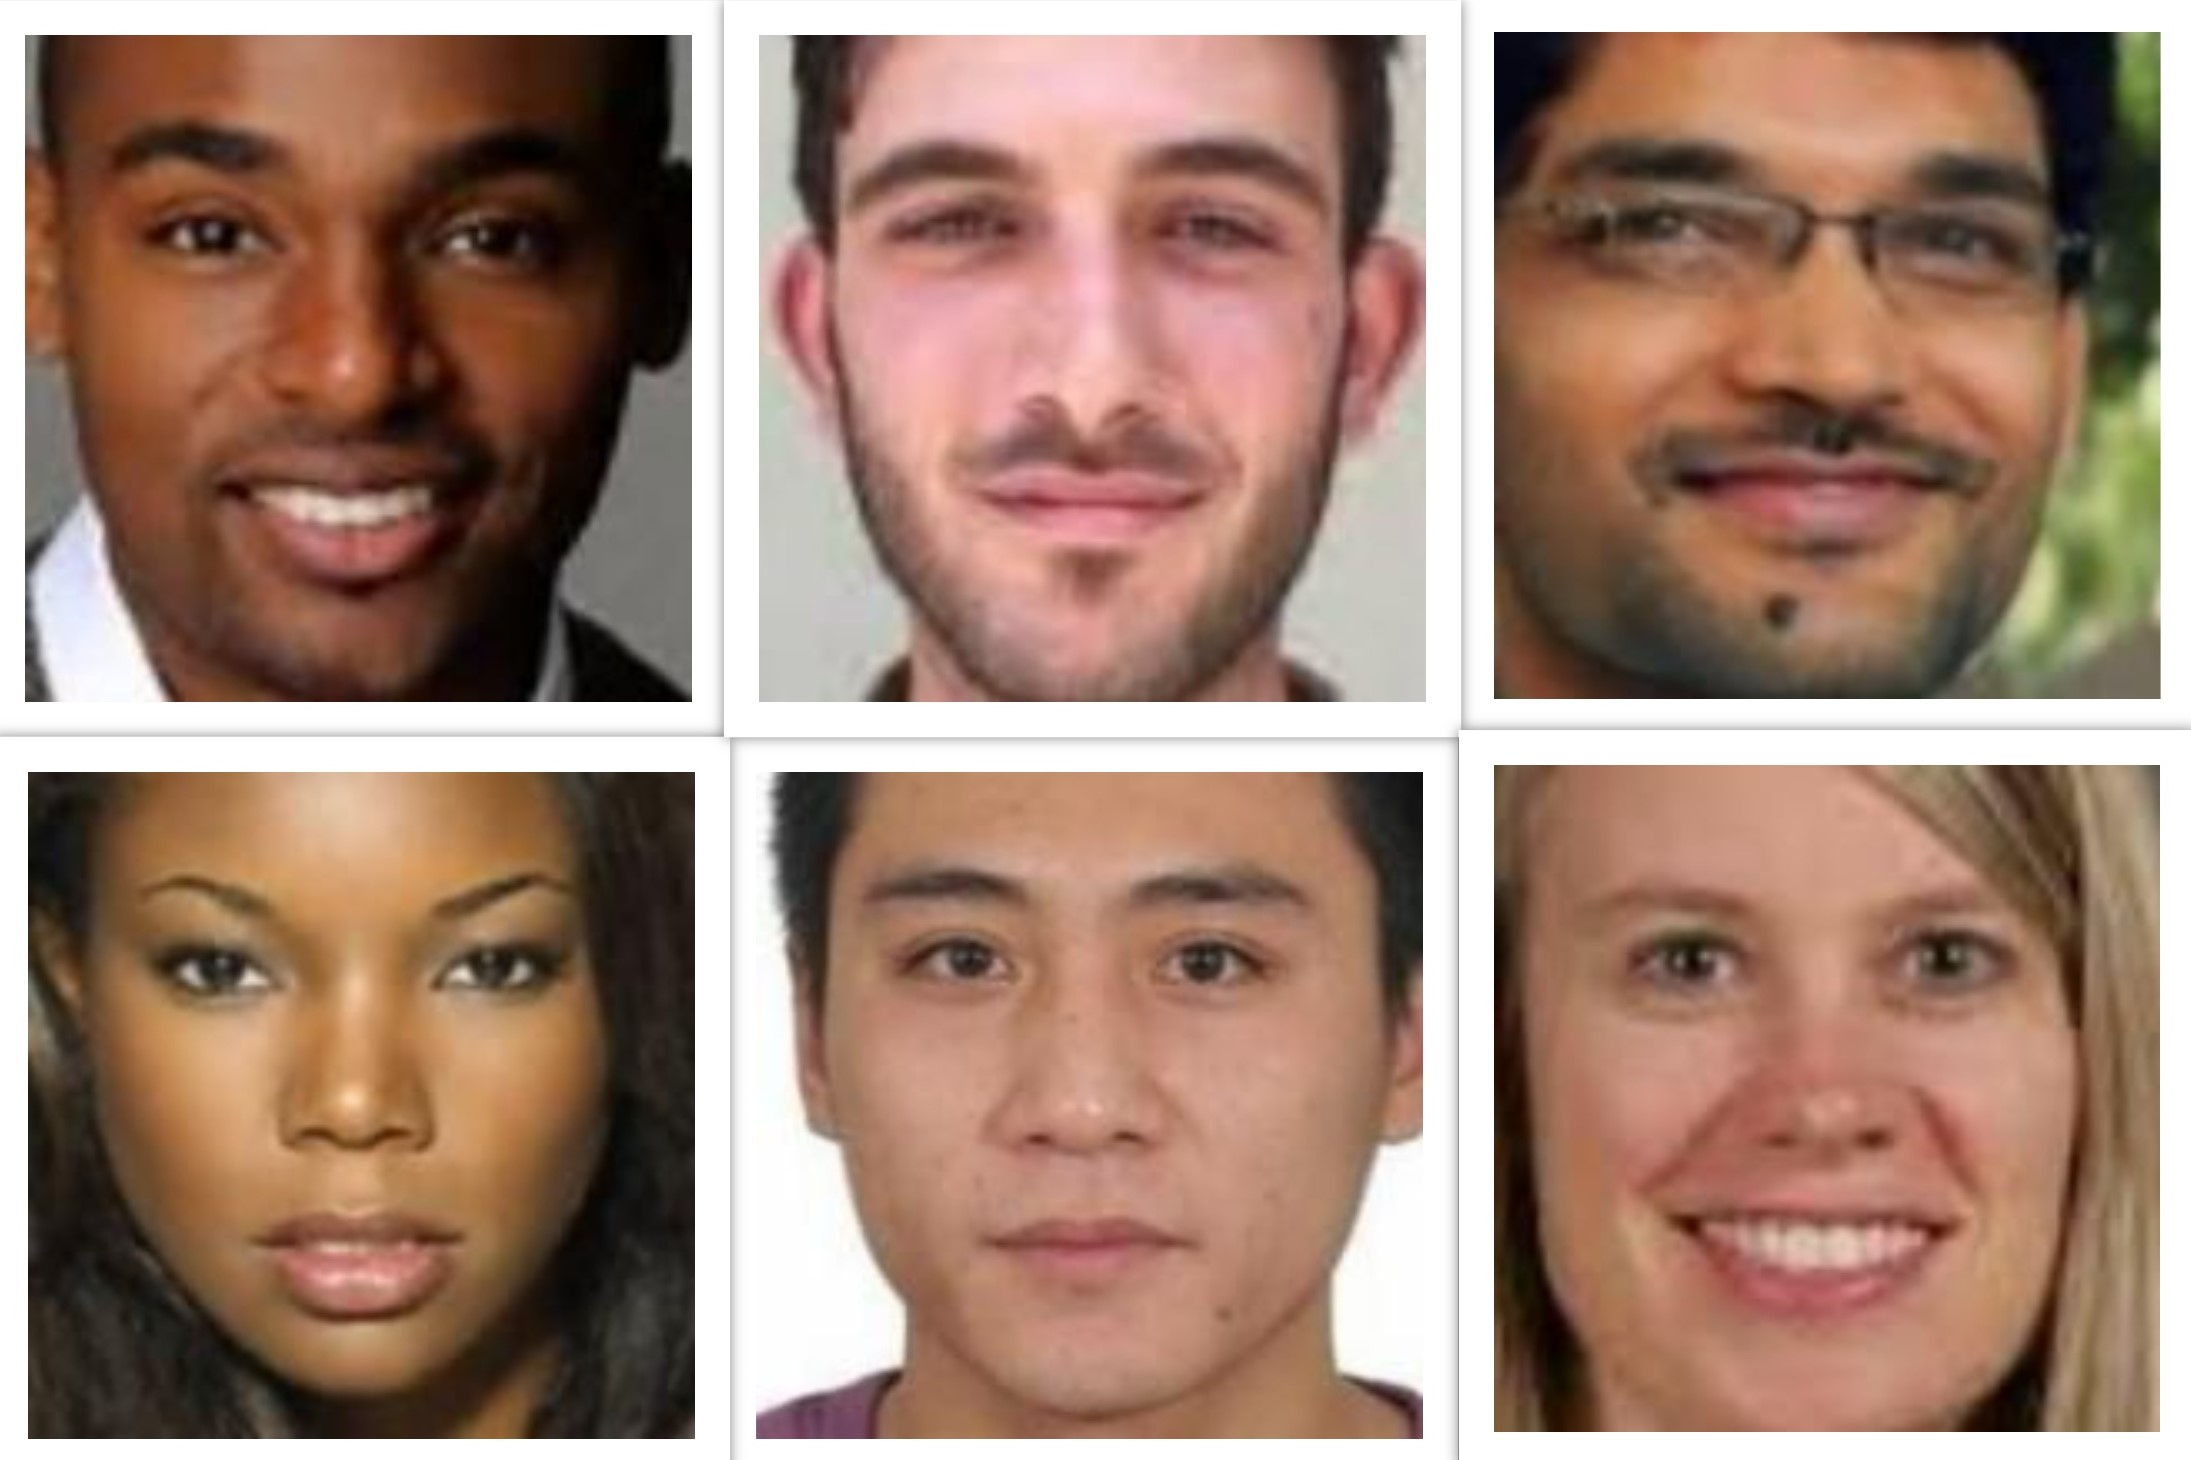
\includegraphics[width=\textwidth]{Arduino/sampldata}
	\caption{Beispielbilder aus dem Datensatz UTKFace
		\index{Datensatz!UTKFace}  }
	\label{UTKFace}
\end{figure}


